\documentclass[xcolor=dvipsnames,10pt]{beamer}

\mode<presentation> {\usetheme{Singapore}}
\usepackage{pgfpages}

%\setbeamercovered{transparent} 
\usepackage[english]{babel}
\usepackage[latin1]{inputenc}
\usepackage{times,amsfonts}
\usepackage[T1]{fontenc}
\setlength{\parskip}{\baselineskip}
% Or whatever. Note that the encoding and the font should match. If T1
% does not look nice, try deleting the line with the fontenc.

%\usecolortheme{sidebartab}
\setbeamertemplate{itemize item}[triangle]



\usepackage{calc}
\usepackage{environ}
\newcommand{\halfmargin}{0.0001\paperwidth}


\RequirePackage{booktabs,colortbl,ulem}

\usepackage{animate}
\RequirePackage{booktabs,colortbl,gensymb}
\setlength{\parskip}{\baselineskip}

\usepackage{calc}
\usepackage{environ}

% \newcommand{\halfmargin}{0.0001\paperwidth}


\NewEnviron{wideframe}[1][]{%
\begin{frame}{#1}
\makebox[\textwidth][c]{
\begin{minipage}{\dimexpr\paperwidth-\halfmargin-\halfmargin\relax}
\BODY
\end{minipage}}
\end{frame}
}


\DeclareMathOperator{\stdev}{stdev}
\DeclareMathOperator{\var}{var}
\DeclareMathOperator{\cov}{cov}
\DeclareMathOperator{\corr}{corr}
\DeclareMathOperator{\prob}{prob}
\DeclareMathOperator{\n}{n}
\DeclareMathOperator{\N}{N}
\DeclareMathOperator{\Cov}{Cov}

\newcommand{\hlf}{\frac{1}{2}}
\newcommand{\bi}{\begin{itemize}}
\newcommand{\ei}{\end{itemize}}
\newcommand{\im}{\item}
\newcommand{\D}{\mathrm{d}}
\newcommand{\E}{\mathrm{e}}
\newcommand{\mye}{\ensuremath{\mathsf{E}}}
\newcommand{\myreal}{\ensuremath{\mathbb{R}}}
\newcommand{\bq}{\begin{equation}}
\newcommand{\eq}{\end{equation}}
\newcommand{\eqdef}{\;\buildrel \text{d{}ef}\over = \;}
\newcommand{\xstar}{\buildrel *\over X}
\newcommand{\pmax}{p^{\text{max}}}
\newcommand{\qmax}{q^{\text{max}}}
\newcommand{\bfr}{\begin{frame}}
\newcommand{\bfrp}{\begin{frame}[plain]}
\newcommand{\efr}{\end{frame}}
\newcommand{\F}{\mathcal{F}}
\newcommand{\FF}{\mathbb{F}}
\newcommand{\ve}{\varepsilon}
\newcommand{\lh}{\hat{\lambda}}
\definecolor{mycolor}{gray}{0.8}
\definecolor{mymaincolor}{rgb}{0.6862745098039216,0.9333333333333333,0.9333333333333333}
\newcommand{\alr}[1]{\textcolor{blue}{#1}}
\definecolor{LightCyan}{rgb}{0.88,1,1}
\newcommand{\yel}{\cellcolor{yellow}}
\newcommand{\blue}{\cellcolor{SkyBlue}}
\newcommand{\gr}{\cellcolor{SpringGreen}}
\newcommand{\pink}{\cellcolor{pink}}
\newcommand{\apr}{\cellcolor{Apricot}}
\newcommand{\tve}{\tilde{\varepsilon}}
\newcommand{\tw}{\tilde{w}}
\newcommand{\ttth}{\tilde{\theta}}
\newcommand{\te}{\tilde{e}}
\newcommand{\ts}{\tilde{s}}
\newcommand{\tx}{\tilde{x}}
\newcommand{\ty}{\tilde{y}}
\newcommand{\tv}{\tilde{v}}
\newcommand{\tp}{\tilde{p}}
\newcommand{\tF}{\tilde{F}}
\newcommand{\tf}{\tilde{f}}
\newcommand{\tZ}{\tilde{Z}}
\newcommand{\ow}{\overline{w}}
\newcommand{\lb}{\left[}
\newcommand{\rb}{\right]}
\newcommand{\lp}{\left(}
\newcommand{\rp}{\right)}
\newcommand{\tm}{\tilde{m}}
\newcommand{\tc}{\tilde{c}}
\newcommand{\tz}{\tilde{z}}
\newcommand{\str}[1]{\textcolor{blue}{\sout{#1}}}
\newcommand{\tr}{\widetilde{R}}
\newcommand{\tR}{\widetilde{\mathbf{R}}}
\newcommand{\bms}{\begin{multline*}}
\newcommand{\ems}{\end{multline*}}
\newcommand{\bas}{\begin{align*}}
\newcommand{\eas}{\end{align*}}
\newcommand{\qr}{\mathbb{Q}}
\newcommand{\IMAGES}{/home/kerry/Dropbox/Images}
\newcommand{\tX}{\tilde{X}}
\newcommand{\tY}{\tilde{Y}}

\author{\vskip 0.5in \small Kerry Back \\BUSI 521--ECON 505\\ Rice University \\Spring 2022}
%\institute{Rice University\\ Spring 2019}
\date[]






\title{\vskip 0.5in Day 4}
\subtitle{Stochastic Discount Factors II}


\begin{document}

%%%%%%%%%%%%%%%%%%%%%%%%%%%%%%%%%%%%%%%%%%%%%%%%%%%%%%%%%%%%%%%%%%%%%%%

\begin{frame}[plain]
  \titlepage
\end{frame}

%%%%%%%%%%%%%%%%%%%%%%%%%%%%%%%%%%%%%%%%%%%%%%%%%%%%%%%%%%%%%%%%%%%%%%%

\begin{frame}{Today}

\bi
\im Arbitrage pricing
\im Finite state model
\im Complete markets
\im Projections and the Hansen-Jagannathan bound
\ei
\end{frame}

\section{Arbitrage}
\subsection{}

\begin{frame}{Pricing by Arbitrage}
    `Pricing by arbitrage' means assuming the existence of an SDF and then deriving values, without assuming utility maximization.
    
    To derive values, we need the SDF to be unique, which requires market completeness (more later).
    
    The phrase `by arbitrage' is used, because the existence of arbitrageurs, who cause arbitrage opportunities to be eliminated, is sufficient to imply the existence of an SDF.
    
    In contrast, `equilibrium pricing' means assuming utility maximization by an investor with some assumed utility function.
\end{frame}
\end{frame}

\bfr\frametitle{Arbitrage Opportunities}
An arbitrage opportunity is a portfolio $\theta$ satisfying
\begin{itemize}
\item It doesn't cost anything: $p'\theta \leq 0$,
\item It doesn't leave you with a liability: $\sum_{i=1}^n \theta_i\tilde{x}_i \geq 0$ with probability~1, and
\item You're paid to take it, either at date 0 or date 1: either $p'\theta<0$ or $\sum_{i=1}^n \theta_i\tilde{x}_i > 0$ with positive probability (or both).
\end{itemize}

Absence of arbitrage opportunities implies the existence of a strictly positive SDF (separating hyperplane theorem).
\end{frame}

\bfr\frametitle{Law of One Price}
Include the risk-free asset (if it exists) as one of the $n$ assets.

The LOP means that each portfolio payoff comes at a unique cost:
$$\sum_{i=1}^n \theta_i \tx_i = \sum_{i=1}^n \hat{\theta}_i \tx_i \quad \Rightarrow \quad \sum_{i=1}^n \theta_i p_i = \sum_{i=1}^n \hat{\theta}_i p_i$$
 Equivalently, a zero-payoff portfolio must have a zero cost:
$$\sum_{i=1}^n \theta_i \tx_i = 0 \quad \Rightarrow \quad \sum_{i=1}^n \theta_i p_i = 0$$
There is an SDF (in finite-state or finite-variance model) if and only the LOP holds.
\end{frame}




\section{Finite States}
\subsection{}
\bfr\frametitle{Arrow Securities}
Assume there are $k<\infty$ states of the world. We can regard any random variable as a $k$ vector.  

The definition of an SDF $m \in \myreal^k$ is that for each asset payoff $x \in \myreal^k$ with price $p$, we have
$$p \ = \ \sum_{j=1}^k m_jx_j \prob_j $$
We can set $q_j = m_j\prob_j$ to obtain
$$p \ = \ \sum_{j=1}^k x_jq_j$$
Definition: An Arrow security is an asset that pays a unit of consumption in a particular state and zero in all other states.
$q_j$ is the price of the Arrow security.  It is also called a state price.

\end{frame}

\bfr\frametitle{Finite State Model}
 $n$ assets and $k$ states.  $X = n \times k$ matrix of asset payoffs.  Each asset is a row.  

 Vector of asset prices is $p \in \myreal^n$
 
 Portfolio payoff is $X'\theta \in \myreal^k$ for $\theta \in \myreal^n$

State price vector is a $q \in \myreal^k$ such that $Xq = p$

SDF is a vector of state prices divided by probabilities

\end{frame}

\section{Complete Markets}
\subsection{}

\bfr\frametitle{Complete Markets}
A market is complete if every random variable (or every finite-variance random variable or \ldots ) is the payoff of some portfolio:
$$(\forall\, \tw) \quad (\exists\, \theta) \quad \sum_{i=1}^n \theta_i \tx_i = \tw$$

If there are infinitely many states of the world (continuous distributions) and only finitely many assets, then the market cannot be complete.  Also, moral hazard and adverse selection limit markets.
But completeness is a useful benchmark.

Completeness implies uniqueness of the SDF: if $\tm$ and $\tilde{n}$ are both SDFs in a complete market, then $\mye[\tm\tx] = \mye[\tilde{n}\tx]$ for all random variables $\tx$, which means that $\tm-\tilde{n}$ is orthogonal to every random variable $\tx$, which implies that $\tm-\tilde{n}=0$ (a.s.).
\end{frame}

\begin{frame}{Finite States with Complete Markets}
    Completeness in the finite-state model means that for all $w \in \myreal^k$, there exists a portfolio $\theta \in \myreal^n$ such that $X'\theta = w$.  
    
    In other words, the range space of the operator $\theta \mapsto X'\theta$ is all of $\myreal^k$.  This is equivalent to: the rank of $X$ beng $k$.  It requires $n \ge k$.
    
Recall that a state price vector is $q \in \myreal^k$ such that $Xq=p$.

If the market is complete, we can calculate the unique vector of state prices (and thereby the unique SDF) via
$$X'Xq = X'p \quad \Rightarrow \quad q = (X'X)^{-1}X'p$$
If $n=k$, then $q = X^{-1}p$.
\end{frame}

\begin{frame}{Example}
$R_f=1.1$.  Two states.  One risky asset with payoff of 120 in first state and 90 in second.  Two states are equally probable.

What is $X$?  What is the payoff of a portfolio in terms of $X$?  Is the market complete?  If so, what is the unique state price vector and the unique SDF?
    \end{frame}
    
\section{Projections}
\subsection{}

\begin{frame}{Multiple SDFs}
Real markets are incomplete, which implies there are multiple (actually, an infinite number of) SDFs.

It is useful to understand the structure of the set of SDFs.  Here is the basic idea.  Suppose $\tve$ is a random variable that is orthogonal to all returns, meaning $\mye[\tr\tve]=0$ for all returns $\tr$.

Suppose $\tm$ is an SDF.  Then, $\tm+\tve$ is also an SDF.  Why?

We will show that there is a unique SDF $\tm_p$ that is the payoff of some portfolio of assets (we say it is `in the span of the assets.').  

The set of SDFs is the set of random variables $\tm_p + \tve$ where $\tve$ is orthogonal to all returns.

\end{frame}


\bfr\frametitle{Orthogonal Projections}
\begin{center}
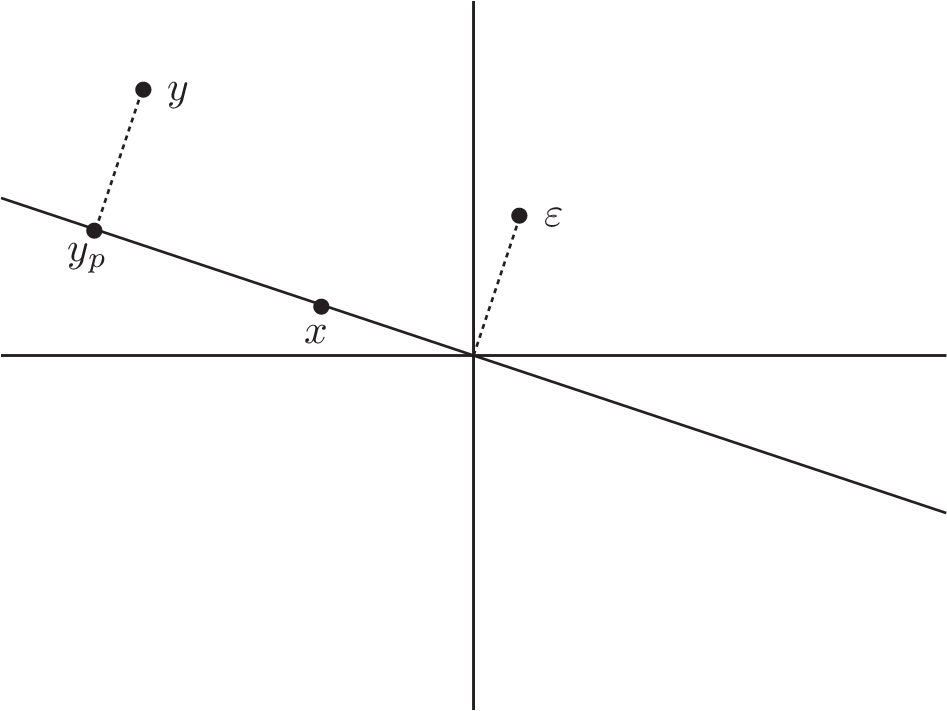
\includegraphics[scale=.9]{Images/fig3_1.png}
\end{center}
\vskip -2\baselineskip
\small $y_p$ is the orthogonal projection of~$y$ onto the line spanned by~$x$.  Specifically, $y=y_p+\varepsilon$, where $y_p$ is spanned by~$x$ (that is, $y_p=bx$ for some constant~$b$) and~$\varepsilon$ is orthogonal to~$x$ (that is, the inner product of~$\varepsilon$ and~$x$ is zero).
\end{frame}

\bfr\frametitle{Projecting SDFs}
Assume all asset payoffs have finite variances and the LOP holds.  Then there is an SDF with finite variance.  We will project all SDFs onto the span of the assets (the projection $\tm_p$ is unique).

 Let $\tX$ denote the column vector with $\tx_i$ as its $i$--th element.  The projection is spanned by $\tX$, meaning, for some $\theta$,
$$\tm_p = \sum_{i=1}^n \theta_i \tx_i = \tX'\theta$$

 The orthogonal projection is defined by the residual $\tve = \tm - \tm_p$ being orthogonal to the $\tx_i$, meaning $\mye[\tve\tx_i]=0$ for all assets $i$.  Equivalently, $\mye[\tX(\tm-X'\theta)]=0$.
\end{frame}

\bfr\frametitle{A Formula for $\tm_p$}
\begin{align*}
\mye[\tX(\tm-\tX'\theta)]=0 \quad &  \Rightarrow \quad \mye[ \tilde{X} \tilde{m} ] = \mye[ \tilde{X}\tilde{X}']\theta \\ \\
\quad &\Rightarrow \quad \theta = \mye[ \tilde{X}\tilde{X}']^{-1}\,\mye[ \tilde{X} \tilde{m} ]\label{4_theta} \\ \\
\quad &\Rightarrow \quad  \tilde{m}_p = \mye[ \tilde{X} \tilde{m} ]'\mye[ \tilde{X}\tilde{X}']^{-1}\tilde{X}\\ \\
\quad &\Rightarrow \quad  \tilde{m}_p = p'\mye[ \tilde{X}\tilde{X}']^{-1}\tilde{X}
\end{align*}
\end{frame}

\bfr\frametitle{An Example}
\vskip -\baselineskip
\begin{center}
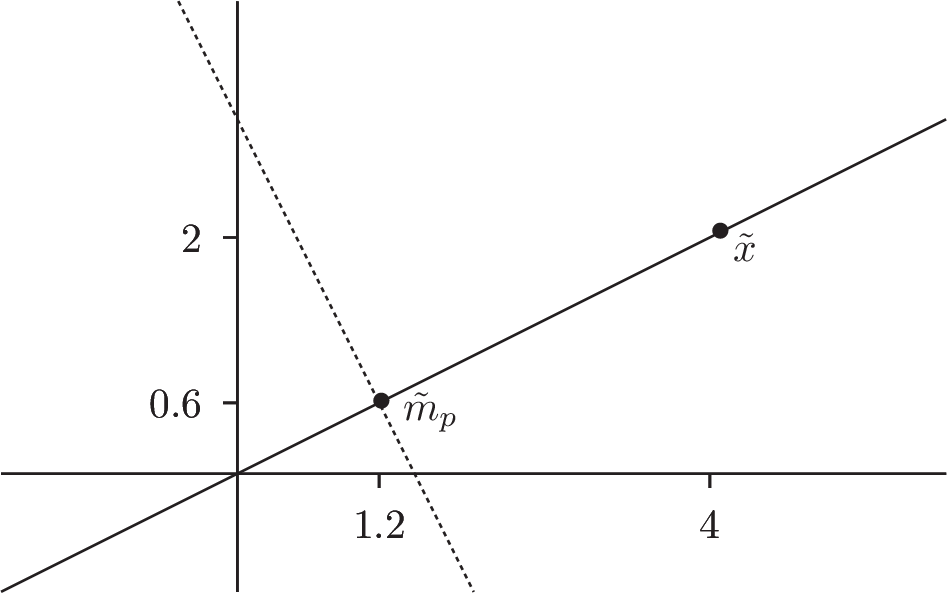
\includegraphics[scale=.7]{Images/fig3_2.png}
\end{center}
\vskip -\baselineskip
\scriptsize There are two states of the world, and they are equally likely.  There is no riskfree asset.  There is a single asset, and it pays~4 in the first state and~2 in the second.  That is, $\tilde{x}=(x_1,x_2)=(4,2)$.  The price of the asset is $p=3$.  

An SDF is any vector $(m_1,m_2)$ satisfying the equation $(1/2)x_1m_1 + (1/2)x_2m_2 = p$, which is equivalent to $2m_1 + m_2 = 3$.  

The span of the assets is the set $\{(y_1,y_2)\mid (y_1,y_2) = \theta (x_1,x_2) \text{\, for some~$\theta$}\}$ and is shown as the solid line.  

The set of SDFs is the dotted line.  The intersection of the set of SDFs with the span of the assets is the SDF $\tilde{m}_p = (6/5,3/5)$. 
\end{frame}


\section{HJ Bound}\subsection{}

\bfr\frametitle{Hansen-Jagannathan Bound with a Risk-Free Asset}
 For any SDF $\tm$ and any return $\tr$,
$$R_f\stdev(\tilde{m})\ \geq \ R_f\stdev(\tilde{m}_p) \ \geq \ \frac{|\mye[\tilde{R}]-R_f|}{\stdev(\tilde{R})}$$
The right-hand side is the absolute value of the Sharpe ratio of $\tr$.

 We can reject an asset pricing model if it implies an SDF that is not sufficiently volatile.  
 For example, SDFs based on consumption growth can be rejected because of the low volatility of consumption growth (the equity premium puzzle).  
More to come on this.

\end{frame}

\bfr\frametitle{Proof of $\stdev(\tilde{m})\geq  \stdev(\tilde{m}_p)$}
 $\cov(\tm_p,\tve) = \mye[\tm_p\tve] - \mye[\tm_p]\mye[\tve] = 0$ because
\bi
\im $\tve$ is orthogonal to span of assets, hence orthogonal to $\tm_p$
\im $\tve$ is orthogonal to $R_f$, hence has mean zero
\ei

Therefore,
\begin{align*}
\var(\tm) \ = \ \var(\tm_p+\tve) &\ = \ \var(\tm_p) + 2\cov(\tm_p,\tve) + \var(\tve) \\
&\ = \ \var(\tm_p) + \var(\tve) \\
 & \ \geq \ \var(\tm_p)
\end{align*}

\end{frame}

\end{document}